\subsection{Reconstructing and evaluating small objects}
\label{sec:small-method}
We study how instance-level instructions and a visual inventory affect
small-object reconstruction in AHa-3D (Figure~\ref{fig:system}, bottom left).
A \emph{target} is an annotated CA-1M box, and an \emph{instance} is a
set of reconstructed mesh parts with a common identifier.

\textbf{All objects} switches AHa-3D from its major-object setting to its
all-object setting (\texttt{precise}). The prompt requires a distinct
identifier for each visible item so that it can move independently of its support.

\begin{figure}[t]
\centering
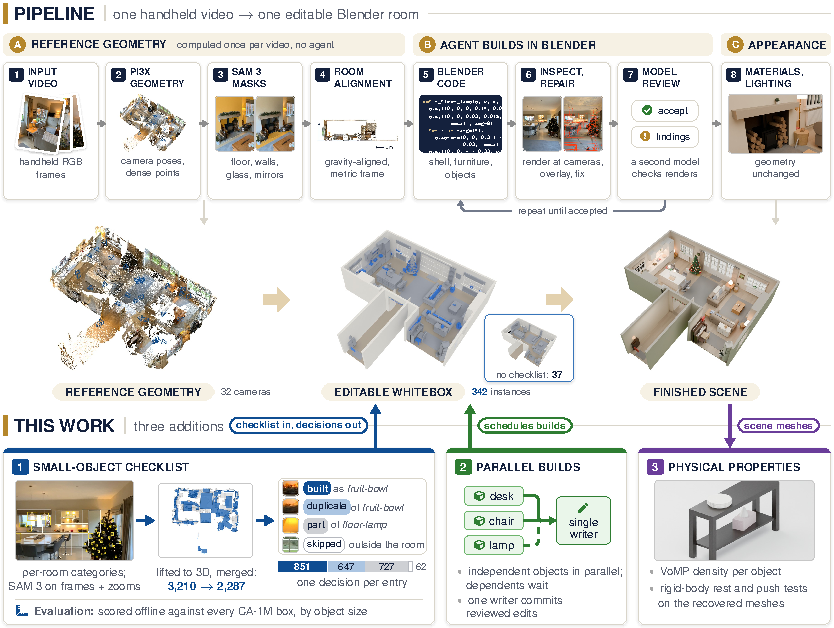
\includegraphics[width=\linewidth]{figures/system-pipeline.pdf}
\caption{\textbf{System overview.} Top: AHa-3D~\cite{aha3d} computes a
reference geometry from a handheld video, an agent authors the room in
Blender against renders from the video's cameras, and an optional pass adds
materials. Middle: one held-out room at each stage; instances under 50\,cm
are blue, and the inset is the same room built without the checklist.
Bottom: our additions, a detector checklist for small objects
(Section~\ref{sec:small-method}; the four entries are real, and the bar
counts the agent's decisions on all 2{,}287 entries of six held-out rooms),
concurrent object builds (Section~\ref{sec:architecture}) and physical
properties (Section~\ref{sec:physics-plan}).}
\label{fig:system}
\end{figure}

\textbf{Inventory} pairs Boxer's predicted 3D boxes and categories~\cite{boxer}
with crops from the video. The agent builds each listed item or explains an
omission, and can still build items Boxer missed. Two further variants let
this agent call an image-to-mesh model,
\href{https://huggingface.co/tencent/Hunyuan3D-2mini}{Hunyuan3D-2mini}~\cite{hunyuan3d2}, for
every object under 50\,cm (\textbf{Required generation}) or at its own
discretion (\textbf{Selective generation}); a generated mesh that fails a
check of silhouette, 3D points, dimensions and support is replaced by
primitives.

\textbf{Revised inventory.}
To improve coverage below 20\,cm, we adapt SceneRig's detection
stage~\cite{scenerig}. A language model extends a fixed category list
with categories observed in eight frames. SAM~3~\cite{sam3} segments them in
full-resolution frames and in nine overlapping zoomed windows, keeping
window-only detections that appear in at least two frames. MoGe-2
depth~\cite{moge2}, rescaled to the reference geometry, lifts each mask to a
3D box. Boxes are then moved onto the surface below them, and similar boxes
of one category share a size.

\textbf{Checklist} uses the revised inventory. We merge same-category
entries when their 3D intersection over union (IoU) exceeds 0.4 or their
centers lie within one fifth of the shorter box diagonal. Across the six
held-out rooms, this reduces 3{,}210 entries to 2{,}287 (Boxer yields 364).
To account for redundant detections, the agent labels each entry as
\emph{built} (a separate instance), \emph{duplicate} (an existing instance),
\emph{part} (of a larger object), or \emph{skipped}. The prompt requires
separate instances for individual objects in stacks or rows. We fixed the
thresholds and prompt on development rooms before held-out evaluation.

\textbf{Camera alignment.}
Each instance is scored as one upright box enclosing its mesh parts. Monocular
video leaves room scale and heading uncertain. For reconstructed and annotated
camera centers $x_i$ and $y_i$ at corresponding frames, the room transform is
\begin{equation}
 T(x)=sR_z(\theta)x+t,\qquad
 (\hat{s},\hat{\theta},\hat{t})=
 \arg\min_{s,\theta,t}\sum_i \lVert T(x_i)-y_i\rVert_2^2 .
 \label{eq:camera-alignment}
\end{equation}
Here $R_z$ rotates about the vertical axis. Object annotations enter only
during offline scoring.

\textbf{Matching and outcomes.}
For an aligned prediction $P$ and target $G$, let $d$ be their center distance,
$L$ the full diagonal of $G$, and $r$ the predicted longest side divided by the
target's longest side. A candidate pair must satisfy $1/3\le r\le 3$ and either
$d\le\max(L/2,0.30\,\mathrm{m})$ or a 3D IoU of at least 0.10.
We greedily match pairs in ascending order of $2d/L+|\log r|$, using
each box at most once regardless of category. A
matched target is \emph{correctly placed} if
\begin{equation}
 d\le\max(0.10\,\mathrm{m},L/4)\quad\text{and}\quad 0.67\le r\le 1.5,
 \label{eq:center-size}
\end{equation}
and \emph{misplaced} otherwise; an unmatched target has no reconstruction.
The three outcomes separate a coverage failure from a placement failure. We
report them by the target's longest side: under 20\,cm, 20 to under 50\,cm,
50\,cm to under 1.5\,m, and larger. Reconstructed instances that match no
target carry no penalty and are reported separately.
Appendix~\ref{app:small} adds a box-overlap criterion and a fit without
scale.
